% Build with: latexmk -pdf main.tex
\documentclass[11pt]{article}

\usepackage[T1]{fontenc}
\usepackage{lmodern}
\usepackage[margin=1in]{geometry}
\usepackage{microtype}
\usepackage{amsmath,amssymb,mathtools}
\usepackage{booktabs}
\usepackage{enumitem}
\usepackage{xcolor}
\usepackage{tikz}
\definecolor{fts}{RGB}{20,70,170}
\usepackage[colorlinks=true,linkcolor=blue!50!black,citecolor=blue!50!black,urlcolor=blue!50!black]{hyperref}

\newcommand{\Th}{\mathsf{Th}}
\newcommand{\hash}{\mathsf{H}}
\newcommand{\Sig}{\mathsf{Sig}}
\newcommand{\Ver}{\mathsf{Ver}}
\newcommand{\OtsSign}{\mathsf{Ots.sign}}
\newcommand{\OtsLeaf}{\mathsf{Ots.leaf}}
\newcommand{\Fold}{\mathsf{Tree.fold}}
\newcommand{\LE}{\mathsf{LE}}
\newcommand{\concat}{\mathbin\Vert}
\newcommand{\idx}{\mathit{idx}}
\newcommand{\pk}{\mathit{pk}}
\newcommand{\sk}{\mathit{sk}}
\newcommand{\rootnode}{\mathit{root}}
\newcommand{\addr}{\mathsf{A}}
\newcommand{\amax}{A_{\max}}

\emergencystretch=1.5em
\setlist[enumerate]{leftmargin=2em, itemsep=4pt}

\title{leanXMSS for Ethereum PQ-Consensus, specification draft}
\author{}
\date{}

\begin{document}
\maketitle

\begin{abstract}
leanXMSS is a stateful hash-based signature scheme: two layers of XMSS~\cite{RFC8391} of height 16 over WOTS$^+$C one-time keys~\cite{HK22C,DKKW25}. Each leaf of the top tree signs the root of one bottom tree, so a key signs at $2^{32}$ leaf indices.
\begin{itemize}
  \item \textbf{Target: NIST security level~1}~\cite{NISTPQC}.
  \item \textbf{Public key: 32 bytes.}
  \item \textbf{Signature: 2404 bytes} ($4+1200+1200$: the leaf index and the two layers).
  \item \textbf{Verification: 201 compressions} of BLAKE2s.
  \item \textbf{Threshold friendly} (Section~\ref{sec:threshold}).
  \item \textbf{Grinding: $\approx2^{20}$ randomizer trials per signature} on average, one compression each.
\end{itemize}
\end{abstract}

\section{Overview}

A key is two layers of Merkle trees of height $h=16$, whose leaves are WOTS$^+$C one-time keys (Figure~\ref{fig:sig}). The top layer is one tree, and its root is the public key. The bottom layer is $2^{16}$ trees, and key $b$ of the top tree signs the root of bottom tree $b$. A leaf index $\idx<2^{32}$ names bottom key $\idx$, in bottom tree $b=\lfloor\idx/2^{16}\rfloor$.

To sign a message $m$ at $\idx$, the signer signs $m$ with bottom key $\idx$ and the root of bottom tree $b$ with top key $b$, and attaches each key's authentication path. The verifier recovers the bottom key's leaf from $m$ and the signature, follows its path to the root of bottom tree $b$, does the same on the top layer, and accepts if it reaches the public key. The scheme is stateful: a leaf index may sign only one message.

\begin{figure}[ht]
\centering
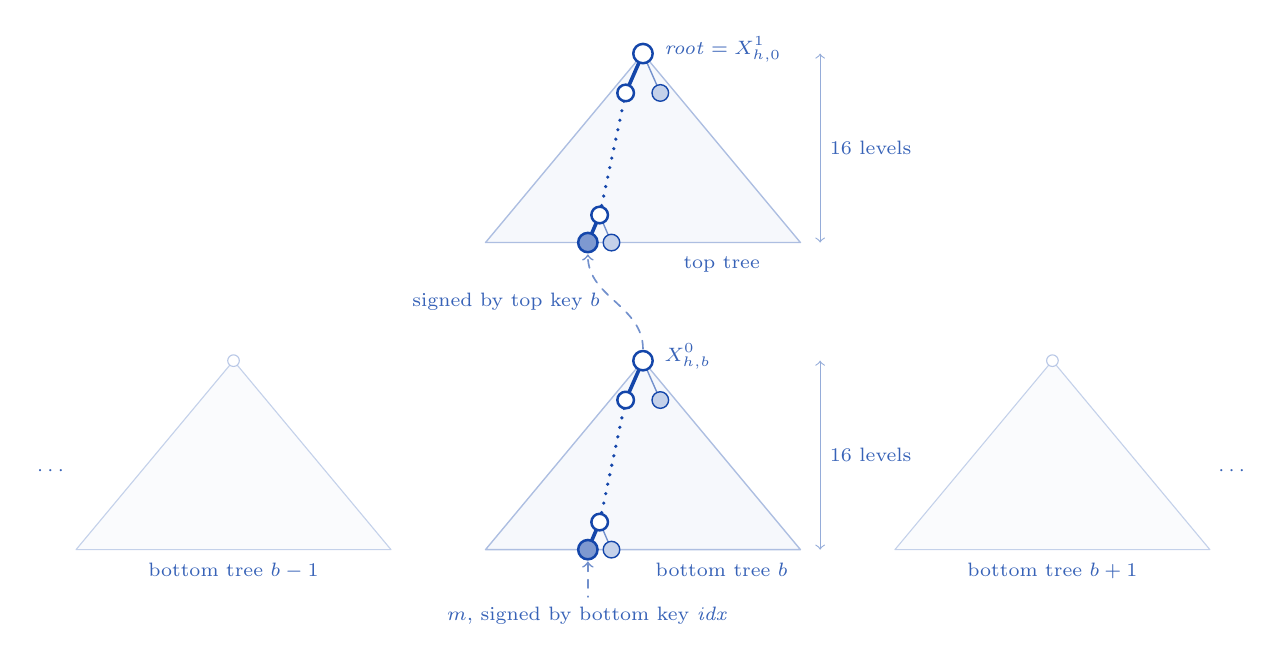
\begin{tikzpicture}[line join=round,line cap=round,
  tri/.style={draw=fts!35,line width=0.5pt,fill=fts!4},
  faded/.style={draw=fts!25,line width=0.4pt,fill=fts!2},
  path/.style={draw=fts,line width=1.3pt},
  gap/.style={draw=fts,line width=1.3pt,dash pattern=on 0pt off 3.5pt},
  edge/.style={draw=fts!60,line width=0.5pt},
  on/.style={circle,draw=fts,line width=0.9pt,fill=white,minimum size=6pt,inner sep=0pt},
  chosen/.style={circle,draw=fts,line width=0.9pt,fill=fts!55,minimum size=7pt,inner sep=0pt},
  auth/.style={circle,draw=fts,line width=0.5pt,fill=fts!25,minimum size=6pt,inner sep=0pt},
  note/.style={font=\scriptsize,text=fts!85}]
% One layer's tree of height 16, base centered at (#1, #2), with the path of one key.
\newcommand{\layer}[2]{
  \draw[tri] (#1-2,#2) -- (#1+2,#2) -- (#1,#2+2.4) -- cycle;
  \draw[edge] (#1-0.4,#2) -- (#1-0.55,#2+0.35) (#1+0.22,#2+1.9) -- (#1,#2+2.4);
  \draw[path] (#1-0.7,#2) -- (#1-0.55,#2+0.35) (#1-0.22,#2+1.9) -- (#1,#2+2.4);
  \draw[gap] (#1-0.55,#2+0.35) -- (#1-0.22,#2+1.9);
  \node[auth] at (#1-0.4,#2) {};
  \node[auth] at (#1+0.22,#2+1.9) {};
  \node[on] at (#1-0.55,#2+0.35) {};
  \node[on] at (#1-0.22,#2+1.9) {};
  \node[on,minimum size=7pt] at (#1,#2+2.4) {};
  \node[chosen] at (#1-0.7,#2) {};
  \draw[fts!45,line width=0.4pt,<->] (#1+2.25,#2) -- node[note,anchor=west] {16 levels} (#1+2.25,#2+2.4);}
\layer{0}{3.9}
\layer{0}{0}
\foreach \c in {-5.2,5.2} {
  \draw[faded] (\c-2,0) -- (\c+2,0) -- (\c,2.4) -- cycle;
  \node[circle,draw=fts!30,line width=0.4pt,fill=white,minimum size=4.2pt,inner sep=0pt] at (\c,2.4) {};}
\node[note] at (-7.5,1) {$\cdots$};
\node[note] at (7.5,1) {$\cdots$};
% Who signs what.
\draw[fts!60,line width=0.6pt,dashed,->] (0,2.55) to[out=90,in=-90] node[note,pos=0.5,anchor=east,xshift=-2pt] {signed by top key $b$} (-0.7,3.75);
\draw[fts!60,line width=0.6pt,dashed,<-] (-0.7,-0.15) -- (-0.7,-0.6) node[note,anchor=north] {$m$, signed by bottom key $\idx$};
% Labels.
\node[note,anchor=west] at (0.15,6.35) {$\rootnode=X^1_{h,0}$};
\node[note,anchor=west] at (0.15,2.45) {$X^0_{h,b}$};
\node[note,anchor=north] at (1,3.85) {top tree};
\node[note,anchor=north] at (1,-0.05) {bottom tree $b$};
\node[note,anchor=north] at (-5.2,-0.05) {bottom tree $b-1$};
\node[note,anchor=north] at (5.2,-0.05) {bottom tree $b+1$};
\end{tikzpicture}
\caption{A signature at leaf index $\idx$, in bottom tree $b=\lfloor\idx/2^{16}\rfloor$, whose leaves are keys $b\,2^{16}$ to $(b+1)2^{16}-1$. On each layer, the verifier recomputes the signing key (dark) and its path to the root (bold) from the siblings the signature carries (shaded, one per level, the 14 middle levels dotted).}
\label{fig:sig}
\end{figure}

\section{Hashing and parameters}

Write $\concat$ for concatenation, $0^k$ for $k$ zero bytes, $\LE_k(z)$ for the $k$-byte little-endian encoding of an integer $z$, and $\LE^{-1}$ for its inverse. Let $\hash$ be unkeyed BLAKE2s-256 (RFC~7693), and $\hash_0,\hash_1$ the first and last 16 bytes of its output. With a 16-byte public parameter $P$ and a 16-byte address $\addr$ (Section~\ref{sec:addresses}),
\[
  \Th(P,\addr,M)=\hash_0(P\concat\addr\concat M).
\]

\begin{center}
\begin{tabular}{@{}lll@{}}
\toprule
Symbol & Value & Meaning\\
\midrule
$v$ & $58$ & chains per one-time key, of positions $0$ to $3$\\
$T$ & $106$ & sum of a codeword's digits\\
$h$ & $16$ & height of each layer's trees\\
$\amax$ & $2^{32}$ & randomizer trials per one-time signature\\
\bottomrule
\end{tabular}
\end{center}

The secret key is a 32-byte seed $S_0$. Every secret derives from $S=\hash(\text{\texttt{leanXMSS}}\concat S_0)$, the hash of the scheme's 8-byte ASCII name then the seed, so that no other scheme derives from the same bytes, and $P=\Th(0^{16},\addr_{\mathrm{param}},S)$. A message $m$ is 32 bytes. The layers are $\ell=0$ (bottom) and $\ell=1$ (top). A leaf index $\idx<2^{32}$ uses key $\idx$ at the bottom, which signs $M=m$, and key $b=\lfloor\idx/2^h\rfloor$ at the top, which signs the 16-byte root $M=X^0_{h,b}$ of bottom tree $b$ (Section~\ref{sec:trees}).

\section{\texorpdfstring{WOTS$^+$C}{WOTS+C}}
\label{sec:ots}

A one-time key is $v$ hash chains of 4 positions. It signs a 16-byte digest that is a codeword, revealing each chain at the position its digit names. The chains of key $e$ on layer $\ell$ are, for $i<v$ and $\mu<3$,
\[
  C_{i,0}=\hash_{i\bmod2}\bigl(P\concat\addr_{\mathrm{prf}}(\ell,e,\lfloor i/2\rfloor)\concat S\bigr),\qquad
  C_{i,\mu+1}=\Th\bigl(P,\addr_{\mathrm{chain}}(\ell,e,\mu),C_{i,\mu}\concat\LE_{16}(i)\bigr),
\]
and its leaf is $X^\ell_{0,e}=\Th(P,\addr_{\mathrm{leaf}}(\ell,e),C_{0,3}\concat\cdots\concat C_{v-1,3})$.

\paragraph{Codewords.} A 16-byte digest $D$ has the digits $x_i=\lfloor\LE^{-1}(D)/4^i\rfloor\bmod4$ for $i<64$. It is a codeword when $x_v=\cdots=x_{63}=0$ and $\sum_{i<v}x_i=T$. Distinct codewords are incomparable, each having a digit smaller than the other's, so the chain values revealed for one codeword never sign another. This replaces the Winternitz checksum.

\paragraph{Signing.} $\OtsSign(\ell,e,M)$ computes
\[
\begin{aligned}
  R_0&=\Th\bigl(P,\addr_{\mathrm{rnd}}(\ell,e),S\concat M\bigr),&
  \rho_c&=\LE_{16}\bigl(\LE^{-1}(R_0)+c\bmod2^{128}\bigr),\\
  D_c&=\Th\bigl(P,\addr_{\mathrm{msg}}(\ell,e),M\concat\rho_c\bigr),
\end{aligned}
\]
takes the least $c<\amax$ for which $D_c$ is a codeword $x$, and returns $\rho=\rho_c$ and the chain values $y_i=C_{i,x_i}$, or $\bot$ if no $c<\amax$ does. It is deterministic. The layout is chosen so that every trial costs exactly one compression: $\rho_c$ is a sum rather than a hash and comes last, so on the bottom layer $P\concat\addr\concat M$ fills the first block, compressed once, and on the top layer the input is one block.

\paragraph{Recovering the leaf.} $\OtsLeaf(\ell,e,M,\rho,y)$ recomputes $D$, returns $\bot$ unless it is a codeword $x$, walks each $y_i$ from position $x_i$ to position $3$, and hashes the ends into the leaf.

\section{Trees}
\label{sec:trees}

On layer $\ell$, for $1\le\lambda\le h$,
\[
  X^\ell_{\lambda,j}=\Th\bigl(P,\addr_{\mathrm{node}}(\ell,\lambda,j),X^\ell_{\lambda-1,2j}\concat X^\ell_{\lambda-1,2j+1}\bigr).
\]
The top layer is one tree, with root $X^1_{h,0}$. The bottom layer is $2^h$ trees whose node indices are global: level $\lambda$ has $2^{2h-\lambda}$ nodes, bottom tree $b$ holds those with $\lfloor j/2^{h-\lambda}\rfloor=b$, and its root is $X^0_{h,b}$ (Figure~\ref{fig:sig}).

The path of key $e$ is $\pi=(\pi_0,\dots,\pi_{h-1})$ with $\pi_\lambda=X^\ell_{\lambda,\lfloor e/2^\lambda\rfloor\oplus1}$, where $\oplus1$ flips the low bit. $\Fold(\ell,e,X,\pi)$ starts from $V_0=X$ and sets $V_{\lambda+1}=\Th(P,\addr_{\mathrm{node}}(\ell,\lambda+1,\lfloor e/2^{\lambda+1}\rfloor),V_\lambda\concat\pi_\lambda)$, the two children swapped when bit $\lambda$ of $e$ is one. It returns $V_h$.


\section{The scheme}

\paragraph{Key generation.} Sample a uniform 32-byte $S_0$ and return $\pk=(X^1_{h,0},P)$ and $\sk=S_0$.

\paragraph{Signing.} $\Sig(\sk,\idx,m)$, with $b=\lfloor\idx/2^h\rfloor$:
\begin{enumerate}
  \item bottom layer: $(\rho^0,y^0)=\OtsSign(0,\idx,m)$, and the path $\pi^0$ of key $\idx$;
  \item top layer: $(\rho^1,y^1)=\OtsSign(1,b,X^0_{h,b})$, and the path $\pi^1$ of key $b$;
  \item return $\sigma=(\idx,\rho^0,y^0,\pi^0,\rho^1,y^1,\pi^1)$, or $\bot$ if either $\OtsSign$ failed.
\end{enumerate}
\textbf{A leaf index must never sign two different messages}: their two codewords would reveal every chain at the smaller of their two positions. The top key $b$ signs only $X^0_{h,b}$, so it signs one message, however many leaf indices of bottom tree $b$ are used.

\paragraph{Serialization.} The public key is $\rootnode\concat P$. A layer's signature is $\rho\concat y_0\concat\cdots\concat y_{v-1}\concat\pi_0\concat\cdots\concat\pi_{h-1}$, $16(1+v+h)=1200$ bytes. The signature is $\LE_4(\idx)$, the bottom layer's, then the top layer's: $4+1200+1200=2404$ bytes.

\paragraph{Verification.} $\Ver((\rootnode,P),m,\sigma)$ rejects unless $\sigma$ is 2404 bytes, parses it as $\idx$, $(\rho^0,y^0,\pi^0)$ and $(\rho^1,y^1,\pi^1)$, and computes
\[
\begin{aligned}
  X&=\Fold\bigl(0,\idx,\OtsLeaf(0,\idx,m,\rho^0,y^0),\pi^0\bigr),\\
  X'&=\Fold\bigl(1,b,\OtsLeaf(1,b,X,\rho^1,y^1),\pi^1\bigr).
\end{aligned}
\]
It accepts exactly when neither $\OtsLeaf$ fails and $X'=\rootnode$.

\paragraph{Verification cost.} A $k$-byte input costs $\lceil k/64\rceil$ compressions. Verification costs, per layer, 2 (bottom) or 1 (top) for the digest, $3v-T=68$ for the chains, 15 for the leaf and 16 for the path: 201 in all.

\paragraph{Signing cost.} Building a tree costs $219\cdot2^h-1$ compressions: per key, 29 for the chain starts, $3v=174$ chain steps and 15 for the leaf, then $2^h-1$ nodes. Key generation builds the top tree, and the signer builds each bottom tree when it first signs in it. A digest is a codeword with probability
\[
  p=[z^{T}](1+z+z^2+z^3)^{v}/2^{128}\approx2^{-20},
\]
so an encoding takes about $2^{20}$ trials on average, one compression each, and all $\amax$ trials fail with probability below $\exp(-2^{11})$. A signature needs one encoding per layer, but the top layer's depends only on the bottom tree, so the signer grinds it once per bottom tree: amortized, a signature costs about $2^{20}$ trials.

\section{Address encoding}
\label{sec:addresses}

Addresses keep the hash inputs of a key distinct. An address is $\mathsf{enc}(\tau,\mu,\mathit{hi},\mathit{lo})=\LE_4(\mathit{lo})\concat\LE_3(\mathit{hi})\concat\LE_1(\tau+32\mu)\concat0^8$, with type $\tau<32$ and $\mu<8$. The top layer sets bit 23 of $\mathit{hi}$: $\mathit{hi}_\ell(a)=a+2^{23}\ell$.
\begin{center}
\begin{tabular}{@{}ll@{\qquad}ll@{}}
\toprule
$\addr_{\mathrm{prf}}(\ell,e,j)$ & $\mathsf{enc}(0,0,\mathit{hi}_\ell(j),e)$ & $\addr_{\mathrm{param}}$ & $\mathsf{enc}(5,0,0,0)$\\
$\addr_{\mathrm{chain}}(\ell,e,\mu)$ & $\mathsf{enc}(1,\mu,\mathit{hi}_\ell(0),e)$ & $\addr_{\mathrm{rnd}}(\ell,e)$ & $\mathsf{enc}(7,0,\mathit{hi}_\ell(0),e)$\\
$\addr_{\mathrm{leaf}}(\ell,e)$ & $\mathsf{enc}(2,0,\mathit{hi}_\ell(0),e)$ & $\addr_{\mathrm{msg}}(\ell,e)$ & $\mathsf{enc}(12,0,\mathit{hi}_\ell(0),e)$\\
$\addr_{\mathrm{node}}(\ell,\lambda,j)$ & $\mathsf{enc}(3,0,\mathit{hi}_\ell(\lambda),j)$ & & \\
\bottomrule
\end{tabular}
\end{center}

\section{Threshold signing}
\label{sec:threshold}

A key can be held by $n$ operators, any $t$ of whom can sign. This section sketches one way to do it, after PRAWNS~\cite{PRAWNS}. It is an example, not part of the scheme.

\paragraph{Idea.} The bottom keys derive their secrets from a context-aware threshold PRF $F$~\cite{PRAWNS}: any $t$ operators can evaluate it, and $t-1$ cannot predict its outputs. Each chain starts at an output of $F$, and the setup publishes the chain's two middle values, each masked with an output of $F$, and its end. A WOTS$^+$C signature reveals one value per chain, which the signers obtain by evaluating $F$ once, or read if it is the end, with no MPC. Signing takes two rounds: one for the randomizer base $R_0$, derived from an output of $F$, and one for the chain values. The top keys only sign bottom roots, so the setup signs them.

\paragraph{Setup.} Either a trusted dealer computes everything in the clear for a lifetime of $L$ bottom trees, or the operators run MPC~\cite{CDI05,GS20} at key generation and once per bottom tree.

\paragraph{Costs.} The public data is 48 bytes per chain: 182\,MB per bottom tree, or 7.3\,GB per year of 12-second slots. With MPC, a bottom tree costs its $2^h\cdot3v\approx1.1\cdot10^7$ chain steps. Each is one compression: 480 additions of 32-bit words, at 31 AND gates each, so a bottom tree takes $1.7\cdot10^{11}$ AND gates. At one bit sent per AND gate~\cite{AFLNO16}, each operator sends about 21\,GB per bottom tree, or 27\,KB/s with 12-second slots.

\bibliographystyle{plain}
\bibliography{refs}

\end{document}
